\pdfbookmark{Parallelization Approaches}{parallelization approaches}
\chapter{Parallelization Approaches}
\label{Parallelization:Sequential}

The section of code which takes more time is the \ttDilepKinFit function. The main objective is to run as many kinematical reconstructions per event, with a slight variation to the particle characteristics, and as they increase the \ttDilepKinFit execution time also increases. So, since it is the critical section of the application, the efforts on performance optimizations will be focused on this portion of the code.

The \ttDilepKinFit workflow can be divided in three main stages. Each event can have an arbitrary number of jets and leptons associated, requiring a minimum of two of each to perform the kinematical reconstruction of the \ttbar system. Events that not fulfill this requirement are discarded in the previous cuts. If there is more than the minimum number of jets and leptons it is necessary to combine them, in pairs of two jets with two leptons, and perform the kinematical reconstruction for every combination possible. Note that their order on the combination is not relevant, reducing the total amount of possible combinations. Then, it is possible to apply a variation to the jets and leptons characteristics, motivated by the reasons explained in section \ref{Motivation}. The variation has a magnitude equivalent to the experimental resolution of the ATLAS detector (which is 5\%) and it is applied to the three momentums and energy of the particles, and causing the need to re-compute other auxiliary parameters to the rest of \ttDilepKinFit. The number of variations to apply to each jet/lepton combination is arbitrary and defined by the user.

\ttDilepKinFit has a main loop, for each jet/lepton combination and for each variation of each combination, where the most intensive computation occurs, which will be explained next, and a final section of code that iterates through all the reconstructions and picks only the best, discarding all the others computed.

Inside the main loop of \ttDilepKinFit is possible to identify three distinct stages of the reconstruction. The first is the variation of the jets and leptons momentums, as explained before. The second stage is the kinematical reconstruction of the \ttbar system, using the varied combinations. It attempts to reconstruct the \ttbar system, presented in section \ref{Motivation} and produces a result (the Top Quarks), which has an computed probability associated to its accuracy. This probability determines the quality of the reconstruction. The third stage is the reconstruction of the Higgs boson, using the results of the kinematical reconstruction. This reconstruction also has a probability associated, and the final quality of the overall reconstruction of the event is given by the multiplication of this probability with the one of the kinematical reconstruction of the \ttbar system. Figure \ref{fig:SeqPipeline} presents the explained workflow of \ttDilepKinFit.

\begin{figure}[!htp]
	\begin{center}
		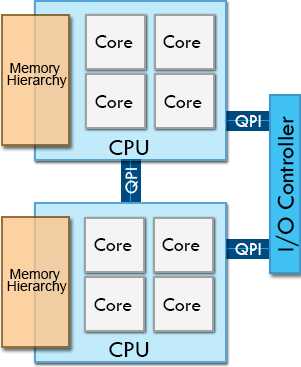
\includegraphics[scale=0.5]{../../common/img/numa_qpi.png}
		\caption{Schematic representation of the \ttDilepKinFit workflow.}
		\label{fig:SeqPipeline}
	\end{center}
\end{figure}

Note that there is data dependencies between loop iterations, since that for chosing the next jet/lepton combination it is necessary to know which combinations were already picked, and between the three stages within the loop. The kinematical reconstruction needs the combination already varied, and the Higgs boson reconstruction needs the result from the kinematical reconstruction in order to chose different particles (since one particle cannot belong to the \ttbar system and the Higgs boson decay). The current workflow is not suitable for parallelization.

A generalist workflow suited for parallelization is presented in figure \ref{fig:ParallelPipeline}. The combinations must be computed, and also all the variations, and their information stored in a data structure, so that the main loop of \ttDilepKinFit is eliminated. Now, each stage of the workflow can have its own loop, which is not represented in the figure since it is considered to be part of the stage itself. By having their own loop, the stages can now be executed in parallel, but maintaining the same data dependencies between stages.

\begin{figure}[!htp]
	\begin{center}
		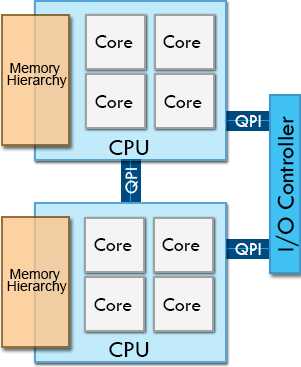
\includegraphics[scale=0.5]{../../common/img/numa_qpi.png}
		\caption{Schematic representation of the \ttDilepKinFit workflow.}
		\label{fig:ParallelPipeline}
	\end{center}
\end{figure}

\pdfbookmark{Shared Memory Parallelization}{shared memory parallelization}
\section{Shared Memory Parallelization}
\label{Parallelization:SharedMem}

The parallel workflow model proposed for this implementation is similar to the generalist previously presented. One challenge to the implementation is that most of the variables are global to the application, and there is no data structure holding the information needed during \ttDilepKinFit, such as the combinations. The computation of the jet/lepton combinations must be kept sequential, since choosing one combination is always dependent on all the previous combinations made and, therefore, cannot be parallelized. The final iteration through all the results, in which the best solution is chose and is ``uploaded'' to global variables, cannot also be parallelized in the current implementation (there is, however, a way to overcome part of this problem that will be explained later). During this chapter a concurrent task is considered to be the subset of a parallel region. The aggregation of all these tasks is the whole parallel region. Figure \ref{fig:SharedMemPipeline} presents the workflow used for this implementation, and is explained next.

\begin{figure}[!htp]
	\begin{center}
		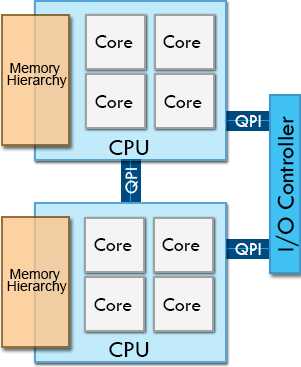
\includegraphics[scale=0.5]{../../common/img/numa_qpi.png}
		\caption{Schematic representation of the \ttDilepKinFit workflow.}
		\label{fig:SharedMemPipeline}
	\end{center}
\end{figure}

In this implementation it does not make any sense to use different tasks for different stages that can be parallel; two of the three steps presented next that can be parallel will be aggregated in the same task, increasing its granularity and reducing the number of synchronizations necessary between tasks. The first step of the new workflow is to create a data structure holding all the combinations and other information associated with them. Each task will pick the respective combination and perform a loop over the subset of the total number of variations. The grain size of the parallel work of each task will be dependent on the total number of combinations times the number of variations per combination (the higher this value the coarser the grains size) and the number of parallel tasks (the higher the number of tasks the thinner the grain size).

The second step, the kinematical reconstruction of the \ttbar system, will be performed within the same task, meaning that there is no synchronization between this and the previous steps among different tasks. The same happens between this and the third step, the Higgs boson reconstruction. By aggregating these three steps the grain size of the tasks is increased, compared to the generalist parallelization model presented before, which benefits their execution on CPU (a lesser number of coarser tasks means that the CPU spends more time performing computations relevant to the application and less time switching context, which is very slow).

As explained before, after these three stages, on the original workflow, there is an iteration through all the solutions and the best is chosen. Instead of saving all the solutions, after each iteration of the loop of the current workflow the solution is compared to the previous and only the best of the two is save. When all tasks finish all their respective iterations, each will have the best solution for the subset of combinations and variations that they processed. A reduction can be made so that the best solution from all the tasks is found. However, another data structure must be created, since the best solution is a set of variables and TLorentzVectorWFlags (from the LipMiniAnalysis library) class instances. The final ``uploading'' of the best solution to global variables is only made by the task with the best solution.

This workflow will have two limitations to the performance scalling, the creation of the data structure holding the combinations and the best solutions and the creation and work sharing between the tasks. Its time increases with the number of combinations and variations and the number of parallel tasks to use.